%%%%%%%%%%%%%%%%%%%%%%%%%%%%%%%%%%%%%%%
% Wenneker Resume/CV
% LaTeX Template
% Version 1.1 (19/6/2016)
%
% This template has been downloaded from:
% http://www.LaTeXTemplates.com
%
% Original author:
% Frits Wenneker (http://www.howtotex.com) with extensive modifications by 
% Vel (vel@LaTeXTemplates.com)
%
% License:
% CC BY-NC-SA 3.0 (http://creativecommons.org/licenses/by-nc-sa/3.0/
%
%%%%%%%%%%%%%%%%%%%%%%%%%%%%%%%%%%%%%%

%----------------------------------------------------------------------------------------
%	PACKAGES AND OTHER DOCUMENT CONFIGURATIONS
%----------------------------------------------------------------------------------------

\documentclass[a4paper,12pt]{memoir} % Font and paper size

%%%%%%%%%%%%%%%%%%%%%%%%%%%%%%%%%%%%%%%%%
% Wenneker Resume/CV
% Structure Specification File
% Version 1.1 (19/6/2016)
%
% This file has been downloaded from:
% http://www.LaTeXTemplates.com
%
% Original author:
% Frits Wenneker (http://www.howtotex.com) with extensive modifications by 
% Vel (vel@latextemplates.com)
%
% License:
% CC BY-NC-SA 3.0 (http://creativecommons.org/licenses/by-nc-sa/3.0/)
%
%%%%%%%%%%%%%%%%%%%%%%%%%%%%%%%%%%%%%%%%%

%----------------------------------------------------------------------------------------
%	PACKAGES AND OTHER DOCUMENT CONFIGURATIONS
%----------------------------------------------------------------------------------------

\usepackage{XCharter} % Use the Bitstream Charter font
\usepackage[utf8]{inputenc} % Required for inputting international characters
\usepackage[T1]{fontenc} % Output font encoding for international characters

\usepackage[top=1cm,left=0cm,right=1cm,bottom=1cm]{geometry} % Modify margins

\usepackage{graphicx} % Required for figures

\usepackage{flowfram} % Required for the multi-column layout

\usepackage[hidelinks]{hyperref} % URLs

\usepackage[usenames,dvipsnames]{xcolor} % Required for custom colours

\usepackage{tikz} % Required for the horizontal rule

\usepackage{enumitem} % Required for modifying lists
\setlist{noitemsep,nolistsep} % Remove spacing within and around lists

\setlength{\columnsep}{\baselineskip} % Set the spacing between columns

% Define the left frame (sidebar)
\newflowframe{0.2\textwidth}{\textheight}{0pt}{0pt}[left]
\newlength{\LeftMainSep}
\setlength{\LeftMainSep}{0.2\textwidth}
\addtolength{\LeftMainSep}{1\columnsep}
 
% Small static frame for the vertical line
\newstaticframe{1.5pt}{\textheight}{\LeftMainSep}{0pt}
 
% Content of the static frame with the vertical line
\begin{staticcontents}{1}
\hfill
\tikz{\draw[loosely dotted,color=RoyalBlue,line width=1.5pt,yshift=0](0,0) -- (0,\textheight);}
\hfill\mbox{}
\end{staticcontents}
 
% Define the right frame (main body)
\addtolength{\LeftMainSep}{1.5pt}
\addtolength{\LeftMainSep}{1\columnsep}
\newflowframe{0.7\textwidth}{\textheight}{\LeftMainSep}{0pt}[main01]

\pagestyle{empty} % Disable all page numbering

\setlength{\parindent}{0pt} % Stop paragraph indentation

%----------------------------------------------------------------------------------------
%	NEW COMMANDS
%----------------------------------------------------------------------------------------

\newcommand{\userinformation}[1]{\renewcommand{\userinformation}{#1}} % Define a new command for the CV user's information that goes into the left column

\newcommand{\cvheading}[1]{{\Huge\bfseries\color{RoyalBlue} #1} \par\vspace{.6\baselineskip}} % New command for the CV heading
\newcommand{\cvsubheading}[1]{{\Large\bfseries #1} \bigbreak} % New command for the CV subheading

\newcommand{\Sep}{\vspace{1em}} % New command for the spacing between headings
\newcommand{\SmallSep}{\vspace{0.5em}} % New command for the spacing within headings

\newcommand{\aboutme}[2]{ % New command for the about me section
\textbf{\color{RoyalBlue} #1}~~#2\par\Sep
}
	
\newcommand{\CVSection}[1]{ % New command for the headings within sections
{\Large\textbf{#1}}\par
\SmallSep % Used for spacing
}

\newcommand{\CVSectionNoSep}[1]{ % New command for the headings within sections
{\Large\textbf{#1}}\par
% \SmallSep % Used for spacing
}

\newcommand{\CVItem}[2]{ % New command for the item descriptions
\textbf{\color{RoyalBlue} #1}\par
#2
\SmallSep % Used for spacing
}

\newcommand{\CVItemNoSep}[2]{ % New command for the item descriptions
\textbf{\color{RoyalBlue} #1}\par
#2
% \SmallSep % Used for spacing
}

\newcommand{\bluebullet}{\textcolor{RoyalBlue}{$\circ$}~~} % New command for the blue bullets
 % Include the file specifying document layout and packages

%----------------------------------------------------------------------------------------
%	NAME AND CONTACT INFORMATION 
%----------------------------------------------------------------------------------------

\userinformation{ % Set the content that goes into the sidebar of each page
\begin{flushright}
% Comment out this figure block if you don't want a photo
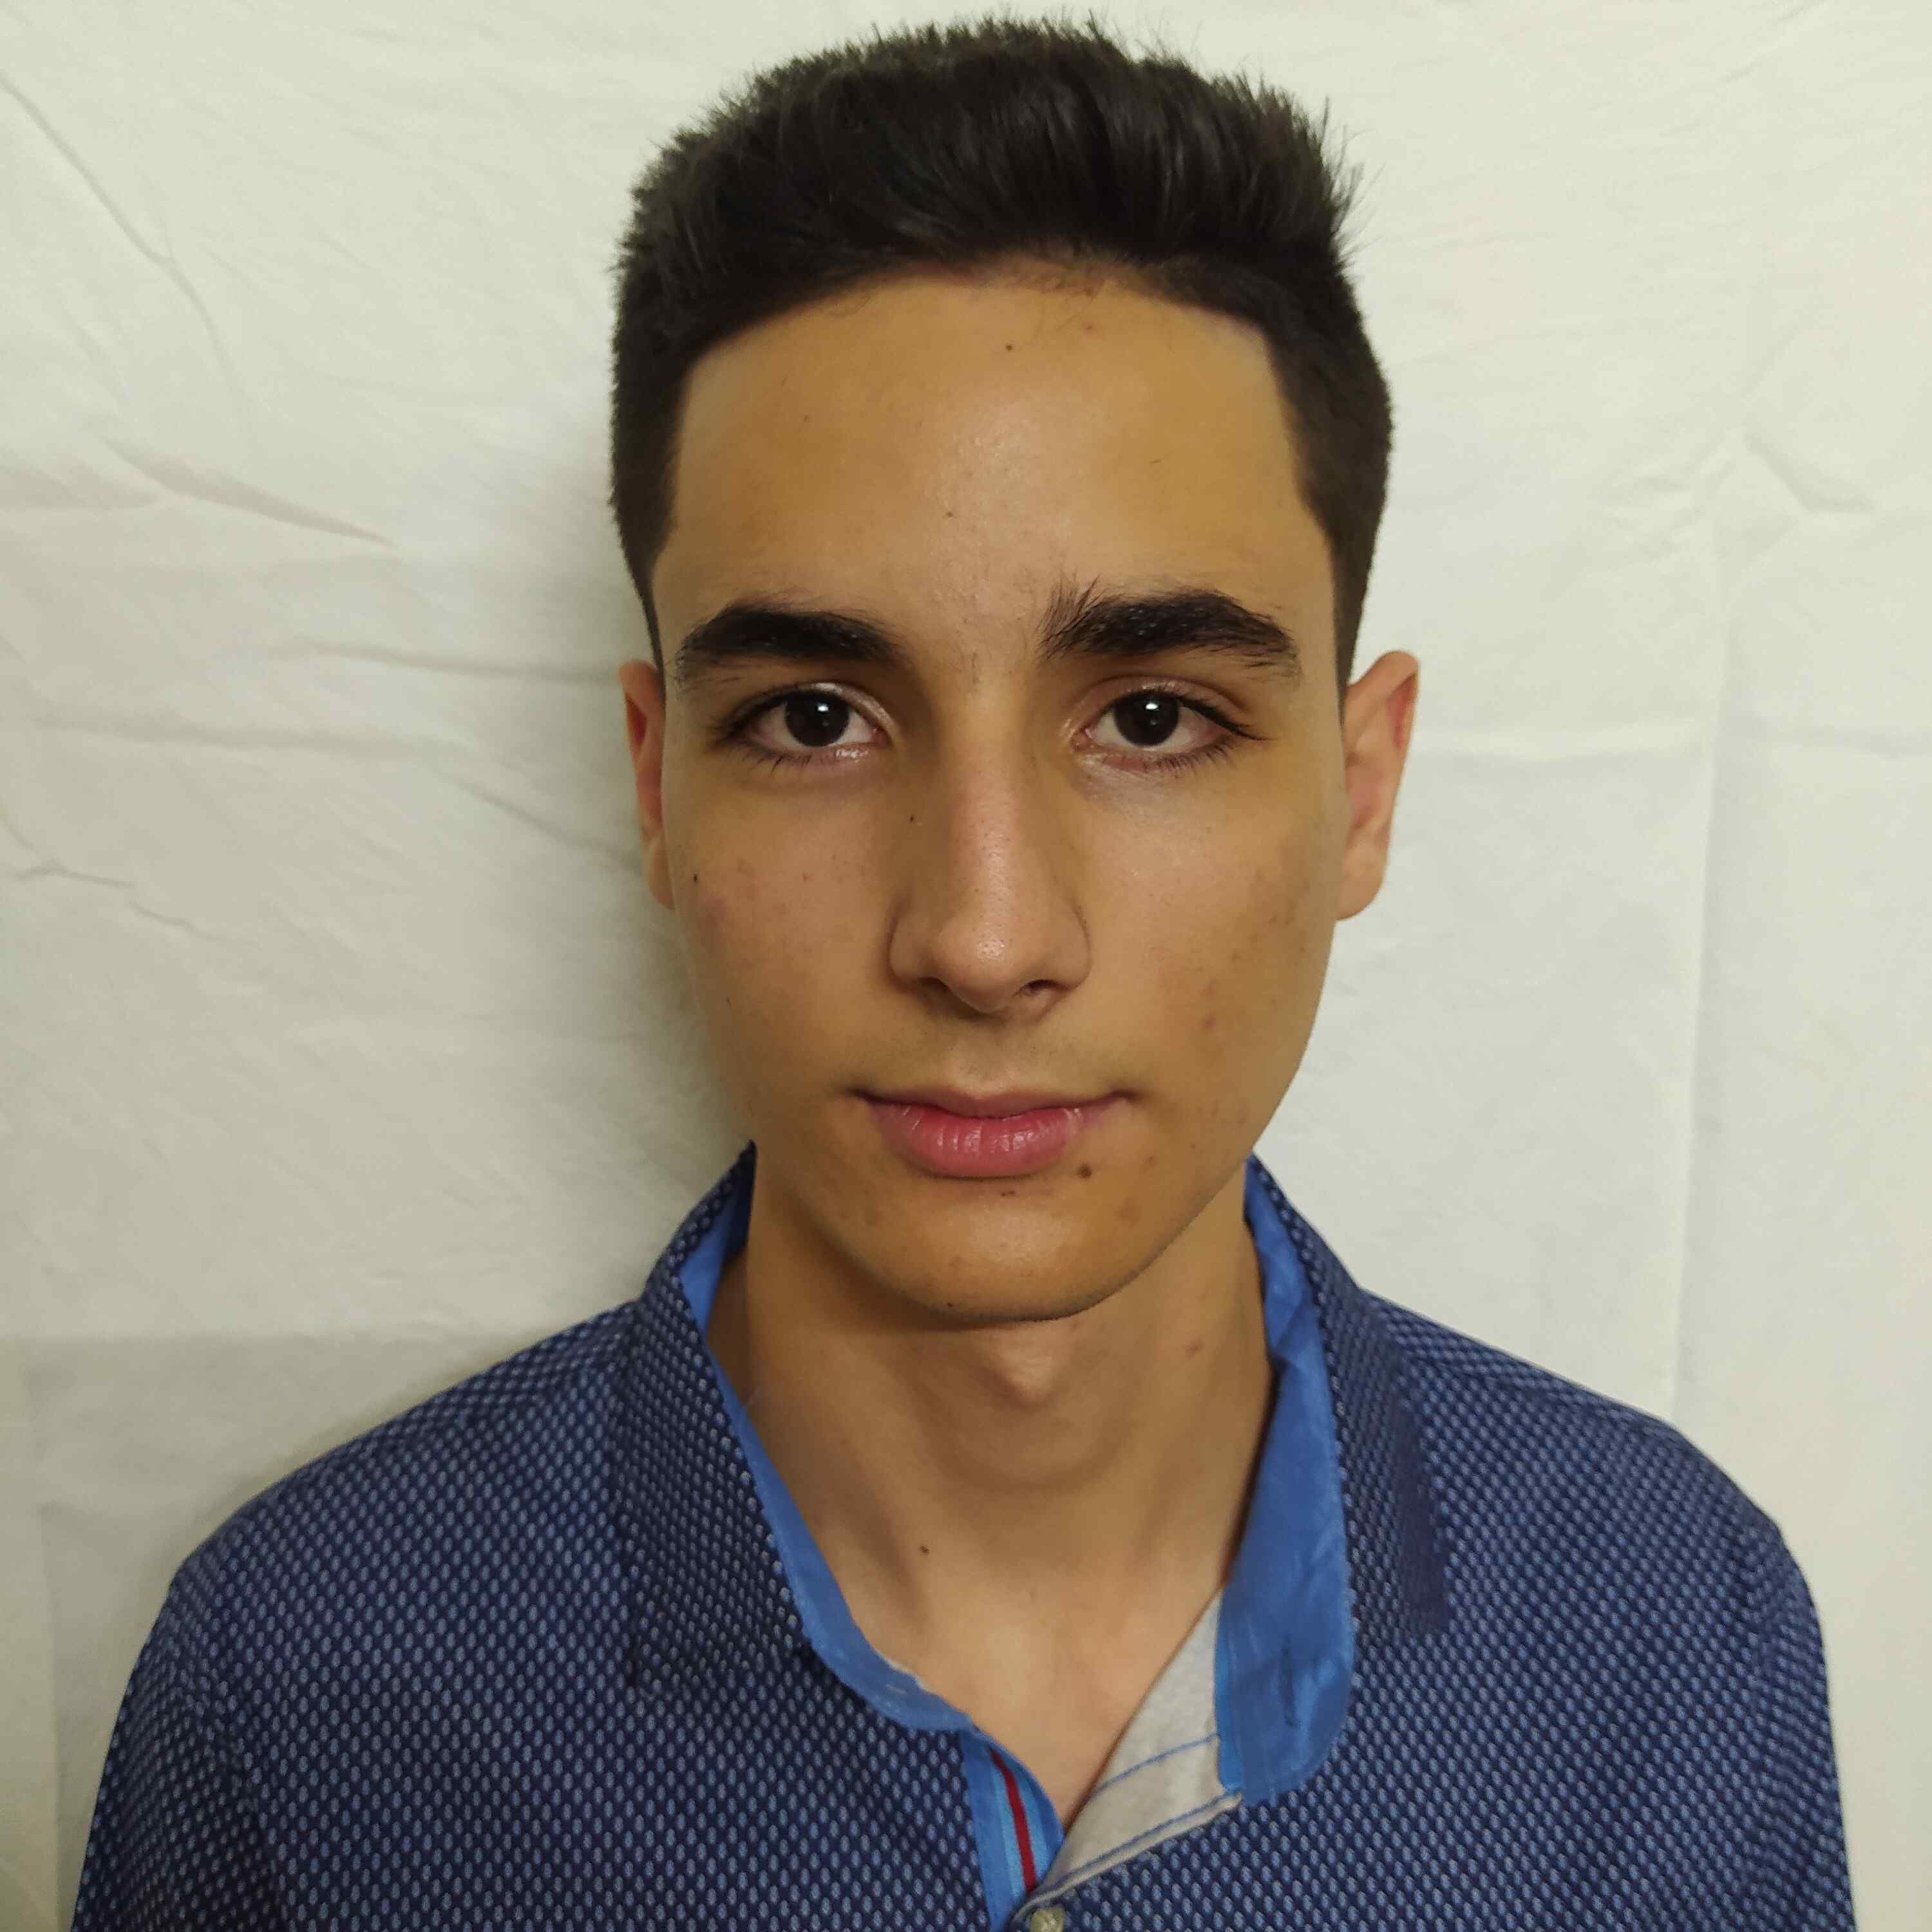
\includegraphics[width=0.6\columnwidth]{photo.jpg}\\[\baselineskip] % Your photo
\small % Smaller font size
Humberto Yusta Gómez \\ % Your name
\Sep % Some whitespace
\href{mailto://humbertoyusta02@gmail.com}{humbertoyusta02@ gmail.com} \\ % Your email address
\Sep % Some whitespace
% \url{www.johnsmith.com} \\ % Your URL
+53 55743975  \\ % Your phone number
\Sep % Some whitespace
\textbf{Dirección} \\
Calle Maceo \#20 \\ % Address 1
Zulueta, Remedios \\ % Address 2
Villa Clara, Cuba \\ % Address 3
\Sep % Some whitespace
GitHub \\
\href{https://github.com/humbertoyusta}{humbertoyusta} \\
\Sep % Some whitespace
LinkedIn \\
\href{https://linkedin.com/in/humberto-yusta-036710212}{humberto-yusta-036710212}
\vfill % Whitespace under this block to push it up under the photo
\end{flushright}
}

%----------------------------------------------------------------------------------------

\begin{document}

\userinformation % Print your information in the left column

\framebreak % End of the first column

%----------------------------------------------------------------------------------------
%	HEADING
%----------------------------------------------------------------------------------------

\cvheading{Humberto Yusta Gómez} % Large heading - your name

\cvsubheading{Estudiante, Programador Competitivo} % Subheading - your occupation/specialization

%----------------------------------------------------------------------------------------
%	ABOUT ME
%----------------------------------------------------------------------------------------

\aboutme{About Me}{Graduado de preuniversitario con cinco años de experiencia 
en programación competitiva. Apasionado por las Matemáticas y las Ciencias de la Computación, 
dedicado al aprendizaje continuo, desarrollo profesional y dispuesto a aprender
nuevas tecnologías y herramientas si surge la necesidad.}

%----------------------------------------------------------------------------------------
%	EXPERIENCE
%----------------------------------------------------------------------------------------

\CVSection{Experience}

%------------------------------------------------

\CVItem{2018 - Presente, \textit{Programador Competitivo}}{
Resultados destacados:
\begin{itemize}
	\item Bronze medal at the International Olympiad in Informatics (IOI 2020) and best Latin-American score.
	\item Master at codeforces.com, Yellow coder at atcoder.jp, Platinum division at usaco.org
	\item Gold medal (3rd place), Bronze medal, and Silver medal at the Ibero-American Competition in Informatics(CIIC) 2020, 2019 and 2018 respectively.
	\item 3rd place at the 2020 ICPC Caribbean Finals (Qualifier), 6th place at 2019 ICPC Caribbean Finals. Participated as guest in both.
	\item Gold medal at the Cuban Informatics Olympiad in 2020, 2019 and 2018. 1st, 2nd and 13th place respectively.
	\item 8th place at the Asia-Pacific Informatics Olympiad 2021 Open Contest.
\end{itemize}
}

%------------------------------------------------

\CVItem{2021 - Present, \textit{Problem Setter \& Trainer}}{Volunteer Work
\begin{itemize}
	\item Author of Codeforces Round \#768 (Div. 1, Div. 2), a competitive programming contest with more than 26000 participants.
	\item Problem setter, tester and staff member in the following contests:
		\begin{itemize}
			\item Ibero-American Competition in Informatics (CIIC) 2022
			\item Ibero-American Competition in Informatics (CIIC) 2021
			\item Cuban Olympiad in Informatics 2022
			\item Cuban Team Selection Contests for the Ibero-American Competition in Informatics in 2021
		\end{itemize}
	\item Author of three educational blogs on codeforces: “XOR Hashing.”, “K-th smallest edge on a tree’s path, a tutorial about its approaches” and
		”Dp with connected components, a simple way to understand it.”.
	\item Personally trained the IOI 2021 Cuba Team for two weeks.
\end{itemize}
}

%------------------------------------------------

\Sep % Extra whitespace after the end of a major section

%----------------------------------------------------------------------------------------
%	EDUCATION
%----------------------------------------------------------------------------------------

\CVSection{Education}

%------------------------------------------------

\CVItem{Sep. 2017 - Aug. 2020, IPVCE Ernesto Che Guevara}{High School Graduate \\
Awarded as one of the best graduates of the Knowledge Contest Training Center.}

%------------------------------------------------

\Sep % Extra whitespace after the end of a major section

%----------------------------------------------------------------------------------------
%	COMMUNICATION SKILLS
%----------------------------------------------------------------------------------------

% \CVSection{Communication Skills}

%------------------------------------------------

% \CVItem{2015, \textit{Oral Presentation}, California Business Conference}{Presented research I conducted for my Masters of Engineering degree.}

%------------------------------------------------

% \CVItem{2014, \textit{Poster}, Annual Business Conference (Oregon)}{As part of the course work for BUS320, I created a poster analyzing several local businesses and presented this at a conference.}

%------------------------------------------------

% \Sep % Extra whitespace after the end of a major section

%----------------------------------------------------------------------------------------
%	SKILLS
%----------------------------------------------------------------------------------------

\CVSectionNoSep{Programming Skills}

%------------------------------------------------

\CVItemNoSep{Programming Languages}
{\begin{tabular}{p{0.2\textwidth} p{0.2\textwidth} p{0.2\textwidth} p{0.2\textwidth}}
\bluebullet C++ &  \bluebullet Java & \bluebullet Typescript & \bluebullet Python\\
\end{tabular}}

%------------------------------------------------

\CVItemNoSep{Development Software}
{\begin{tabular}{p{0.2\textwidth} p{0.2\textwidth} p{0.2\textwidth} p{0.2\textwidth}}
\bluebullet Git &  \bluebullet NestJS & \bluebullet PostgreSQL & \bluebullet Polygon\\
\end{tabular}}

%------------------------------------------------

% \CVItemNoSep{Programming Skills}
% {\begin{tabular}{p{0.2\textwidth} p{0.2\textwidth}}
%  \bluebullet Data Structures and Algorithms &  \bluebullet Mathematical Skills\\
% \end{tabular}}

%------------------------------------------------

% \Sep % Extra whitespace after the end of a major section

%----------------------------------------------------------------------------------------
%	NEW PAGE DELIMITER
%	Place this block wherever you would like the content of your CV to go onto the next page
%----------------------------------------------------------------------------------------

% \clearpage % Start a new page

% \userinformation % Print your information in the left column

% \framebreak % End of the first column

%----------------------------------------------------------------------------------------
%	AWARDS
%----------------------------------------------------------------------------------------

% \CVSection{Awards}

%------------------------------------------------

% \CVItem{2010, \textit{Postgraduate Scholarship}, Cornell University}{Awarded to the top student in their final year of a Bachelors degree.}

%------------------------------------------------

% \Sep % Extra whitespace after the end of a major section

%----------------------------------------------------------------------------------------
%	INTERESTS
%----------------------------------------------------------------------------------------

% \CVSection{Interests}

%------------------------------------------------

% \CVItem{Professional}{Data analysis, company profiling, risk analysis, economics, web design, web app creation, software design, marketing}

%------------------------------------------------

% \CVItem{Personal}{Piano, chess, cooking, dancing, running}

%------------------------------------------------

% \Sep % Extra whitespace after the end of a major section

%----------------------------------------------------------------------------------------

\end{document}
